\documentclass[a4paper,11pt]{article}

\usepackage{a4wide}
\usepackage{microtype}
\usepackage[utf8]{inputenc}
\usepackage[ngerman]{babel}
\usepackage[default,light,semibold]{sourceserifpro}
\usepackage[T1]{fontenc}
\usepackage{mathtools}
\usepackage[dvipsnames]{xcolor}
\usepackage[marginal, norule, perpage]{footmisc}
\usepackage{tabularx}
\usepackage{graphicx}
\usepackage{hyperref}

\renewcommand{\thefootnote}{\Roman{footnote}}
\newcommand{\lskip}{\vspace{1 em} \\}

\def\arraystretch{1.5}

\usepackage{minted}

%settings
\usemintedstyle{lovelace}
\hypersetup{
  colorlinks=true,
  linkcolor=MidnightBlue,
  urlcolor=MidnightBlue
}

%opening
\title{
    \begin{center}
        \Large{Grundlagen Softwareentwicklung}\\
        \rule{0.5\textwidth}{0.1 mm}
    \end{center}
    \vspace{1 em}
    \huge{Nebenläufigkeit} \vspace{0.5 em} \\
    \large{Einführung und Anwendung in Python} \vspace{1.5 em}
}
\author{Markus Reichl}

\begin{document}

\maketitle

\tableofcontents

\section{Einf\"uhrung}
\begin{flushleft}
Die Nebenl\"aufigkeit oder Parallelit\"at (englisch \textit{concurrency}) beschreibt die \textbf{gleichzeitige Abfertigung mehrerer Anweisungen}.
\end{flushleft}
Eine reale Nebenl\"aufigkeit ist gegeben, wenn diese Anweisungen physisch voneinander getrennt sind.
In der Softwareentwicklung wird jedoch meist nur eine scheinbare Parallelit\"at verwendet, diese bezeichnet man als \textbf{Multitasking}.

\subsection{Anwendungsbereiche}
Parallelit\"at wird vor allem dort ben\"otigt wo Aufgaben unabh\"angig voneinander abgearbeitet werden sollen.
Darunter fallen zum Beispiel: \textit{Benutzereingaben}, \textit{Server}, \textit{Sortieralgorithmen}, \dots

\newpage
\section{Multitasking}

Beim Multitasking werden die verschiedenen Prozesse in so kurzen Abst\"anden aktiviert, dass der Eindruck der Gleichzeitigkeit entsteht.
Die Verwaltung dieser Prozesse \"ubernimmt im Betriebssystem der Scheduler.

\begin{figure}[ht]
\centering
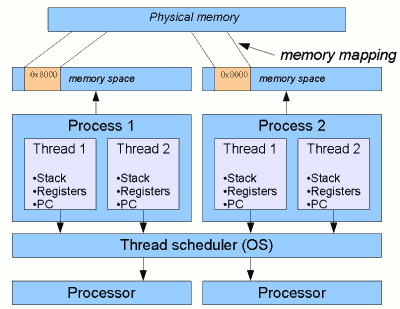
\includegraphics[width=0.55\textwidth]{imgs/ThreadDiagram.png}

\tiny{\textbf{Multitasking am Prozessor}\\ http://www.javamex.com/tutorials/threads/how\_threads\_work.shtml}
\end{figure}

\paragraph{Threads}
Alle Threads innerhalb eines Prozesses teilen sich denselben Adressraum, wodurch sie im Gegensatz zu diesen leichter gestartet, verwaltet und auch zerst\"ort werden k\"onnen.

\paragraph{Prozesse}
Prozesse besitzen einen eigenen Adressraum im Hauptspeicher und bestehen aus mindestens einem Thread\footnote{In Python ist dieser als \mintinline{python}{'__main__'} gekennzeichnet}.
Im Gegensatz zum Threading ist Multiprocessing zwar performanter, jedoch ist auch die Kommunikation zwischen den Prozessen aufwendiger.

\newpage
\subsection{Multithreading}

\paragraph{Thread anhand einer Funktion}
\begin{minted}{python}
import threading

threading.Thread(target=print, args=('Hello World!',)).start()
\end{minted}

\begin{flushleft}
Die k\"urzeste Methode einen neuen Thread zu starten geht \"uber die Klasse \texttt{threading.Thread}.
Diese \"ubernimmt eine Funktion (\mintinline{python}{target=print}) als Objekt, sowie ihre Parameter (\mintinline{python}{args=('Hello World!',)}) als Argumente.
Nach der Instanziierung des Objekts wird die \texttt{run} Methode mittels \texttt{start()} aufgerufen und der Thread gestartet.
\end{flushleft}
Eine Funktion als Thread zu instanziieren ist in den meisten Sprachen der Standard, bei komplexeren Anweisungen wird diese Variante jedoch schnell un\"ubersichtlich.
Besonders in Python hat sich hier eine andere Variante durchgesetzt, bei welcher direkt von \texttt{threading.Thread} geerbt wird.

\paragraph{Thread anhand einer Klasse}
\begin{minted}[linenos]{python}
import threading

class MyThread(threading.Thread):
  def __init__(self):
    super().__init__()

  def run(self):
    print('Hello World!')

thread = MyThread()
thread.start()
\end{minted}
Die eigene Klasse erbt von \texttt{threading.Thread} und ruft im eigenen Konstruktor den des Elternteils auf.
Die zuvor aufgerufene \texttt{run} Methode wird mit der eigenen Funktionalit\"at \"uberschrieben, welche parallelisiert werden soll.
Anstatt nun ein Objekt der Stammklasse zu instanziieren wird die eigene Klasse verwendet und \"uber \texttt{start()} gestartet.

\newpage
\paragraph{Terminierung}
\begin{flushleft}
Sobald ein Thread die \texttt{run} Methode verl\"asst wird dieser automatisch beendet.
H\"aufig sind jedoch andere Anweisungen vom Ergebnis dieses Threads abh\"angig und sollen auf diese warten.
\end{flushleft}
\textbf{Join}\quad
Die \texttt{join()} Methode der Klasse \texttt{threading.Thread} stellt einen blockierenden Aufruf dar.
Dieser wird erst beendet sobald der zugeh\"orige Thread geschlossen wird.
\begin{minted}[linenos, firstnumber=13]{python}
thread.join()

print('Bye!')
\end{minted}
\textbf{Daemons}\quad
W\"ahrend einige Threads den Ablauf direkt beeinflussen sind andere nur im Hintergrund t\"atig.
Diese sollten die Abfertigung des Programms nicht behindern und m\"ussen daher geschlossen werden.\\
Zu diesem Zweck werden in Python sogenannte \textit{daemonic Threads} verwendet.
\vspace{0.5 em}
\begin{minted}[linenos]{python}
import threading

def loop():
  while True:
    print('Hi there')

thread = threading.Thread(target=loop)
# Mark this thread as daemonic
thread.daemon = True
thread.start()
\end{minted}
\textit{Daemonic Threads} werden beendet sobald alle anderen Threads\footnote{Inklusive dem \mintinline{python}{'__main__'} Thread} geschlossen wurden und m\"ussen vor dem Starten mit Hilfe ihres \texttt{daemon} Attributes markiert werden.

\newpage

\subsection{Multiprocessing}
In Python unterscheidet sich der Aufbau von Threads und Prozessen nur geringf\"ugig,
die Grundstruktur bleibt also gleich mit dem einzigen Unterschied, dass \texttt{multiprocessing.Process} anstatt von \texttt{threading.Thread} verwendet wird.

\paragraph{Prozess anhand einer Funktion}
\begin{minted}{python}
import multiprocessing

multiprocessing.Process(target=print, args=('Hello World!',)).start()
\end{minted}

\paragraph*{Prozess anhand einer Klasse}
\begin{minted}[linenos]{python}
import multiprocessing

class MyProcess(multiprocessing.Process):
  def __init__(self):
    super().__init__()

  def run(self):
    print('Hello World!')

process = MyProcess()
process.start()
\end{minted}

\paragraph{Terminierung}
\begin{flushleft}
Die Terminierung erfolgt syntaktisch wie gehabt und \"andert sich von der Funktion her nur geringf\"ugig.
\end{flushleft}
\textbf{Join}\quad
\begin{minted}[linenos, firstnumber=13]{python}
process.join()
\end{minted}
\textbf{Daemons}\quad
\begin{minted}[linenos, firstnumber=7]{python}
process = multiprocessing.Process(target=loop)
# Mark this process as daemonic
process.daemon = True
process.start()
\end{minted}
Prozesse welche als \textit{daemonic} markiert wurden, werden beendet sobald alle anderen Prozesse innerhalb des Programms geschlossen sind.

%\newpage
%
%\section{Interprozesskommunikation}
%\begin{figure}[ht]
%\centering
%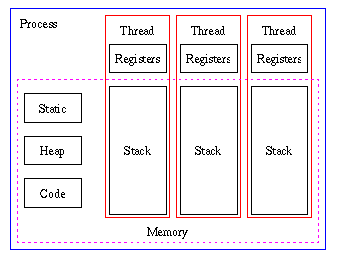
\includegraphics[width=0.5\textwidth]{imgs/MultiStackThread.png}
%
%\tiny{\textbf{Prozesse und Threads im Speicher}\\ https://www.w3.org/People/Frystyk/thesis/MultiStackThread.gif}
%\end{figure}

\end{document}
